% ============================================================
% PHẦN SADGS — Slide 3/8: Clone dựa trên importance đa view (densify_and_clone_structgs)
% ============================================================

\begin{frame}{Nhân bản Gaussian nhỏ nhưng quan trọng (\texttt{densify\_and\_clone\_structgs})}
\footnotesize
\begin{itemize}
    \item Clone dùng cho Gaussian \textbf{còn nhỏ} (chưa cần chia hình học) nhưng đang thiếu mật độ tại vùng có chi tiết -- nhân đôi giữ nguyên scale/rotation/màu, chỉ khác vị trí do phép cộng tensor.
    \item \textbf{3DGS gốc}: điều kiện clone dựa trên \textit{gradient vị trí trung bình} $\lVert\bar g_{xyz}\rVert \ge \tau_{\text{grad}}$ tích luỹ qua backprop -- tín hiệu gián tiếp, nhiễu theo batch view ngẫu nhiên mỗi bước.
    \item \textbf{SADGS}: thay/bổ sung bằng tín hiệu \textbf{tần số -- importance đa view} $\Rightarrow$ Gaussian chỉ được clone khi nhiều góc nhìn khác nhau \textit{đồng thuận} rằng nó cần thêm mật độ, không chỉ 1 view nhiễu tức thời.
\end{itemize}
\vspace{0.2cm}
\small
\centering
\begin{tabular}{lll}
\toprule
\textbf{Tiêu chí} & \textbf{3DGS gốc} & \textbf{SADGS} \\
\midrule
Tín hiệu chọn & Gradient vị trí $\bar g_{xyz}$ & Importance đa view (\texttt{accum\_view\_count}) \\
Điều kiện scale & $\max(\sigma) \le$ \texttt{percent\_dense}$\times$extent & $\max(\sigma) \le$ \texttt{dense}$\times$extent \\
Hàm nhân bản & \texttt{densify\_and\_clone} & \texttt{densify\_and\_clone\_structgs} \\
\bottomrule
\end{tabular}
\end{frame}

% --- Frame 2 ---
\begin{frame}{Điều kiện clone chi tiết}
\footnotesize
Trong \texttt{densify\_and\_prune\_structgs}, một Gaussian được đưa vào tập ứng viên clone khi thoả \textbf{đồng thời} hai lớp điều kiện:
\[
\texttt{clone\_qualifiers} = \big(\max_{\text{axis}}(\sigma) \le \texttt{dense}\times\text{extent}\big), \qquad \texttt{dense}=0.001
\]
\[
\texttt{final\_clone\_mask} = \big(\texttt{grad\_qualifiers} \lor \texttt{full\_split\_mask}\big) \wedge \texttt{clone\_qualifiers}
\]
\begin{itemize}
    \item $\texttt{grad\_qualifiers} = \lVert\bar g_{xyz}\rVert \ge \texttt{grad\_thresh}\,(0.0002)$ -- vẫn giữ tín hiệu gradient chuẩn làm điều kiện cần.
    \item Nhưng để \textbf{thực sự} được nhân bản, còn phải vượt qua bộ lọc \textbf{importance} tính trên toàn cục:
\end{itemize}
\[
\texttt{importance\_score} = \texttt{accum\_view\_count}, \qquad
\texttt{metric\_mask} = \big(\texttt{importance\_score} > \texttt{importance\_score\_threshold}\big),\ \tau{=}0.5
\]
\begin{itemize}
    \item \texttt{accum\_view\_count}: số lần Gaussian được tích luỹ thống kê tần số $\eta$ qua các view liên tiếp -- Gaussian hiếm khi "được nhìn thấy và cần" (đóng góp tần số cao) sẽ có điểm thấp, bị loại dù gradient tức thời cao.
    \item Lệnh gọi thực thi: \texttt{densify\_and\_clone\_structgs(metric\_mask, final\_clone\_mask)} -- bên trong lấy \texttt{selected = metric\_mask \(\wedge\) final\_clone\_mask} rồi copy nguyên các tensor tại các chỉ số đó.
\end{itemize}
\end{frame}

% --- Frame 3 ---
\begin{frame}{Ví dụ số: Gaussian nào được clone?}
\footnotesize
Giả sử extent$=6.0$ $\Rightarrow$ ngưỡng scale $= \texttt{dense}\times\text{extent} = 0.001\times 6.0 = 0.006$; ngưỡng gradient $\texttt{grad\_thresh}=0.0002$; ngưỡng importance $\tau=0.5$ (giả định thang $[0,1]$ đã chuẩn hoá theo số view tối đa quan sát được).
\vspace{0.15cm}
\centering
\begin{tabular}{lccccc}
\toprule
\textbf{GS} & $\max(\sigma)$ & $\lVert\bar g_{xyz}\rVert$ & importance & scale đạt? & \textbf{Kết luận} \\
\midrule
$A$ & $0.004$ & $0.00035$ & $0.72$ & \checkmark & \textbf{Clone} (nhỏ, gradient cao, đa view đồng thuận) \\
$B$ & $0.004$ & $0.00031$ & $0.30$ & \checkmark & Không clone (importance dưới $0.5$ -- chỉ 1--2 view nhiễu) \\
$C$ & $0.009$ & $0.00040$ & $0.85$ & $\times$ & Không clone -- chuyển sang \textbf{split} (đã đủ lớn, xem Slide~4) \\
\bottomrule
\end{tabular}
\vspace{0.2cm}
\begin{itemize}
    \item $A$: thoả cả 3 điều kiện $\Rightarrow$ nhân bản thành 2 Gaussian trùng vị trí, sau đó optimizer sẽ tách chúng dần qua các bước gradient tiếp theo.
    \item $B$: gradient tức thời cao nhưng importance thấp $\Rightarrow$ SADGS coi đây là nhiễu 1 view, \textbf{không} lãng phí ngân sách điểm.
    \item $C$: điều kiện scale không thoả ($\max(\sigma) > 0.006$) $\Rightarrow$ dù importance cao vẫn không clone, mà rơi vào nhánh split.
\end{itemize}
\end{frame}

% --- Frame 4 ---
\begin{frame}{Trực quan hoá trước/sau clone}
\begin{columns}
\begin{column}{0.5\textwidth}
\centering
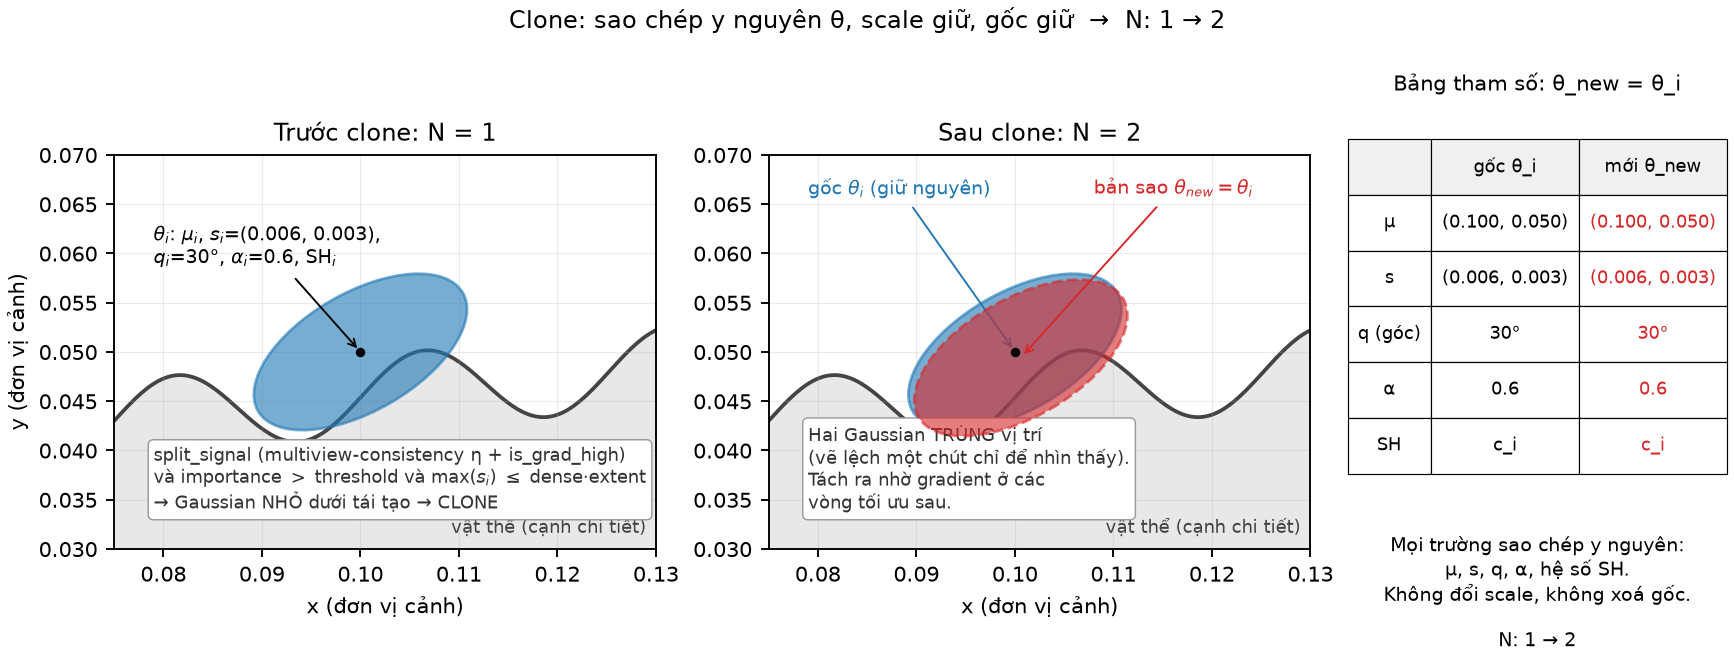
\includegraphics[width=0.95\linewidth]{../BOOK/adc_3dgs/figures/fig_08_clone_before_after.png}
\captionof{figure}{\footnotesize Trước/sau khi clone: Gaussian nhỏ được nhân đôi tại cùng vị trí, giữ nguyên scale/rotation}
\end{column}
\begin{column}{0.5\textwidth}
\footnotesize
\begin{itemize}
    \item Hình minh hoạ \textbf{toy model} tổng quát cơ chế clone (copy nguyên tham số, không đổi hình học) -- \textbf{không} phải render thật từ một cảnh/dataset cụ thể của SADGS.
    \item Sau \texttt{densification\_postfix}: 2 Gaussian con có \textit{cùng} $\mu, \Sigma$, opacity, SH -- chỉ khác nhau ở chỗ chúng là 2 tham số riêng biệt trong optimizer (2 hàng tensor), nên gradient tiếp theo có thể đẩy chúng ra 2 hướng khác nhau.
    \item Bộ đếm \texttt{densify\_count} \textbf{không} tăng khi clone (khác với split) -- vì clone không thay đổi độ mịn hình học, chỉ tăng số lượng điểm phủ vùng đó.
    \item Các bộ tích luỹ tần số (\texttt{accum\_eta}, \texttt{accum\_view\_count}, \texttt{eta\_high/mid/low\_count}) của 2 Gaussian con được khởi tạo lại bằng $0$ -- chúng "bắt đầu lại" quá trình tích luỹ thống kê đa view.
\end{itemize}
\end{column}
\end{columns}
\end{frame}

% --- Frame 5 ---
\begin{frame}{Vì sao clone khác split? Liên hệ sang Slide 4}
\footnotesize
\begin{itemize}
    \item \textbf{Clone}: chỉ \textit{nhân bản} (copy) -- không đổi hình học của từng Gaussian con, không xoay, không co scale. Mục tiêu: tăng \textbf{số lượng điểm} tại vùng mật độ thấp nhưng kích thước Gaussian còn phù hợp với chi tiết ảnh ($\eta$ chưa vượt ngưỡng).
    \item \textbf{Split}: Gaussian đã \textbf{quá lớn} so với chi tiết texture cục bộ ($\max(\sigma) > \texttt{dense}\times\text{extent}$, thường đi kèm $\eta > 1$) $\Rightarrow$ phải \textbf{chia nhỏ hình học} ($\sigma_{\text{new}} = \sigma_{\text{old}}/k$), sinh Gaussian con nhỏ hơn và xoá Gaussian cha.
    \item Cùng dùng chung hàm nội bộ \texttt{densification\_postfix} để nối tensor mới vào optimizer, nhưng khác nhau ở \textbf{có prune Gaussian cha hay không}: clone giữ nguyên cha, split xoá cha (\texttt{prune\_points} sau khi sinh con).
\end{itemize}
\vspace{0.2cm}
\small
\centering
\begin{tabular}{lll}
\toprule
\textbf{Tiêu chí} & \textbf{Clone (Slide 3)} & \textbf{Split (Slide 4)} \\
\midrule
Điều kiện scale & $\max(\sigma)\le\texttt{dense}\times\text{extent}$ & $\max(\sigma) > \texttt{dense}\times\text{extent}$ \\
Hình học con & Giống hệt cha & Chia nhỏ theo $k=\lceil\sqrt{\eta}\rceil$/trục \\
Gaussian cha & Giữ lại & Bị prune (xoá) \\
\texttt{densify\_count} & Không đổi & Tăng $+1$ (kế thừa cha) \\
\bottomrule
\end{tabular}
\end{frame}
